\chapter{Sprint 1 : Enhancements and Integrations}
\setcounter{secnumdepth}{0}

\section{Introduction}
In this chapter, we cover the first sprint of the Aermax project, focusing on the key enhancements and features we implemented to improve the platform.
\setcounter{secnumdepth}{2} 
\section{Major Features and Enhancements}
This section details the major features and enhancements introduced during the first sprint of the Aermax project. Each item listed in the sprint backlog was carefully selected to address critical needs and provide significant improvements to the platform's functionality and user experience.
\subsection{Sprint Backlog Detail}
Below is a detailed representation of our sprint backlog, showcasing the major tasks we committed to delivering in Sprint 1. We fixed around \textbf{26+ bugs, feature enhancements,and new features }in Sprint 1. Below, we're going to share some of them. The biggest changes that we can discuss are highlighted below the blue colored line in the table.
\begin{longtable}{ | m{0.15\textwidth} | m{0.2\textwidth} | m{0.25\textwidth} | m{0.1\textwidth} | m{0.16\textwidth} | }
    \caption{Detailed Sprint Backlog} \\
    \hline
    \textbf{Type} & \textbf{Title} & \textbf{Description} & \textbf{Priority} & \textbf{Estimation} \\
    \hline
    \endfirsthead
    \hline
    \textbf{Type} & \textbf{Title} & \textbf{Description} & \textbf{Priority} & \textbf{Estimation} \\
    \hline
    \endhead
    \hline
    \endfoot
    \endlastfoot
    \rowcolor{blue!20} 
    Feature & Dynamic Equipment List & The ticket describes an issue with a dynamic equipment list system where equipment items are grouped and managed. & High & 40h \\
    \hline
    Feature & Implement User Authentication System & Allow subcontractors to self-register on the platform. & High & 12h \\
    \hline
    \rowcolor{blue!20} 
    Enhancement & Adjust Feedback Notification & Update feedback functionality to include notifications in teams. & Medium & 8h \\
    \hline
    Enhancement & Set Dynamic Project Status & Dynamically set project status based on packet statuses. & High & 2h \\
    \hline
    Enhancement & Add Field to User Edit & Include additional fields in the user edit form. & Medium & 1h \\
    \hline
    Feature & Set Default Calendar View & Remember last selection for default calendar view using localStorage. & Medium & 1h \\
    \hline
    Enhancement & Restrict Project Creation & Prevent subcontractors from creating new projects. & High & 1h \\
    \hline
    Enhancement & Remove Team Types & Remove unnecessary team types from the app to streamline functionality. & Low & 1h \\
    \hline
    Feature & Calendar View with New Filters & Implement new filters for the calendar view for better UX. & High & 40h \\
    \hline
    Feature & Implement Google Maps URL Generation & Generate Google Maps URLs for address visualization in subcompany user view. & Medium & 4h \\
    \hline
    Bug & Overhaul User Access Restrictions & Fix critical access restrictions and bugs for subcompany users. & High & 1h \\
    \hline
    \rowcolor{blue!20} 
    Feature & Overhaul the Role System & Revise the role system to clarify permissions and responsibilities. & High & 1h \\
    \hline
    Feature & Automate Username Generation & Auto-generate usernames during self-registration. & Medium & 1h \\
    \hline
    Feature & Remember Date Filters for Calendar & Implement a feature to remember date filters for the calendar. & Low & 1h \\
    \hline
    Feature & Overhaul the Project Status & Update project status features and adjust status enums and filters. & High & 1h \\
    \hline
    Bug & Fix Read-Only State of User Edit Form & Correct the issue with the user edit form being read-only for admins. & Medium & 1h \\
    \hline
    Bug & Remove Duplicate Aggregated Phases & Remove any duplicate instances of aggregated phases in the system. & High & 1h \\
    \hline
    \rowcolor{blue!20} Enhancement & Enhance Working Packets UI \& UX & Improve the UI and UX for working packets. & Medium & 16h \\
    \hline
\end{longtable}

\subsection{Dynamic Equipment Design}
To effectively transition from a static to a dynamic equipment list, we need to carefully design the system architecture. The following sections provide a detailed overview of the class structure and interactions.
\subsubsection{Dynamic Equipment List issues}
The Dynamic Equipment List feature was previously implemented as a static list. This static list required manual updates and did not reflect real-time changes to the equipment database. The key characteristics of the static implementation included:
\begin{itemize}
    \item Manual updates to the equipment list.
    \item Limited flexibility and responsiveness to changes.
    \item High maintenance overhead due to frequent updates.
\end{itemize}

\subsubsection{Issues with Static Implementation}
The static implementation had several drawbacks:
\begin{itemize}
    \item \textbf{Scalability:} As the number of equipment items grew, maintaining the static list became increasingly cumbersome.
    \item \textbf{Real-time Updates:} Any changes to the equipment database were not immediately reflected in the list, leading to potential inconsistencies.
    \item \textbf{User Experience:} Users could not rely on the list for up-to-date information, which impacted their ability to make informed decisions.
\end{itemize}

As illustrated in Figure \ref{fig:static_equipment_list}, subcontractors were limited to only checking the checkboxes for the available equipment.

\begin{figure}[H]
    \centering
    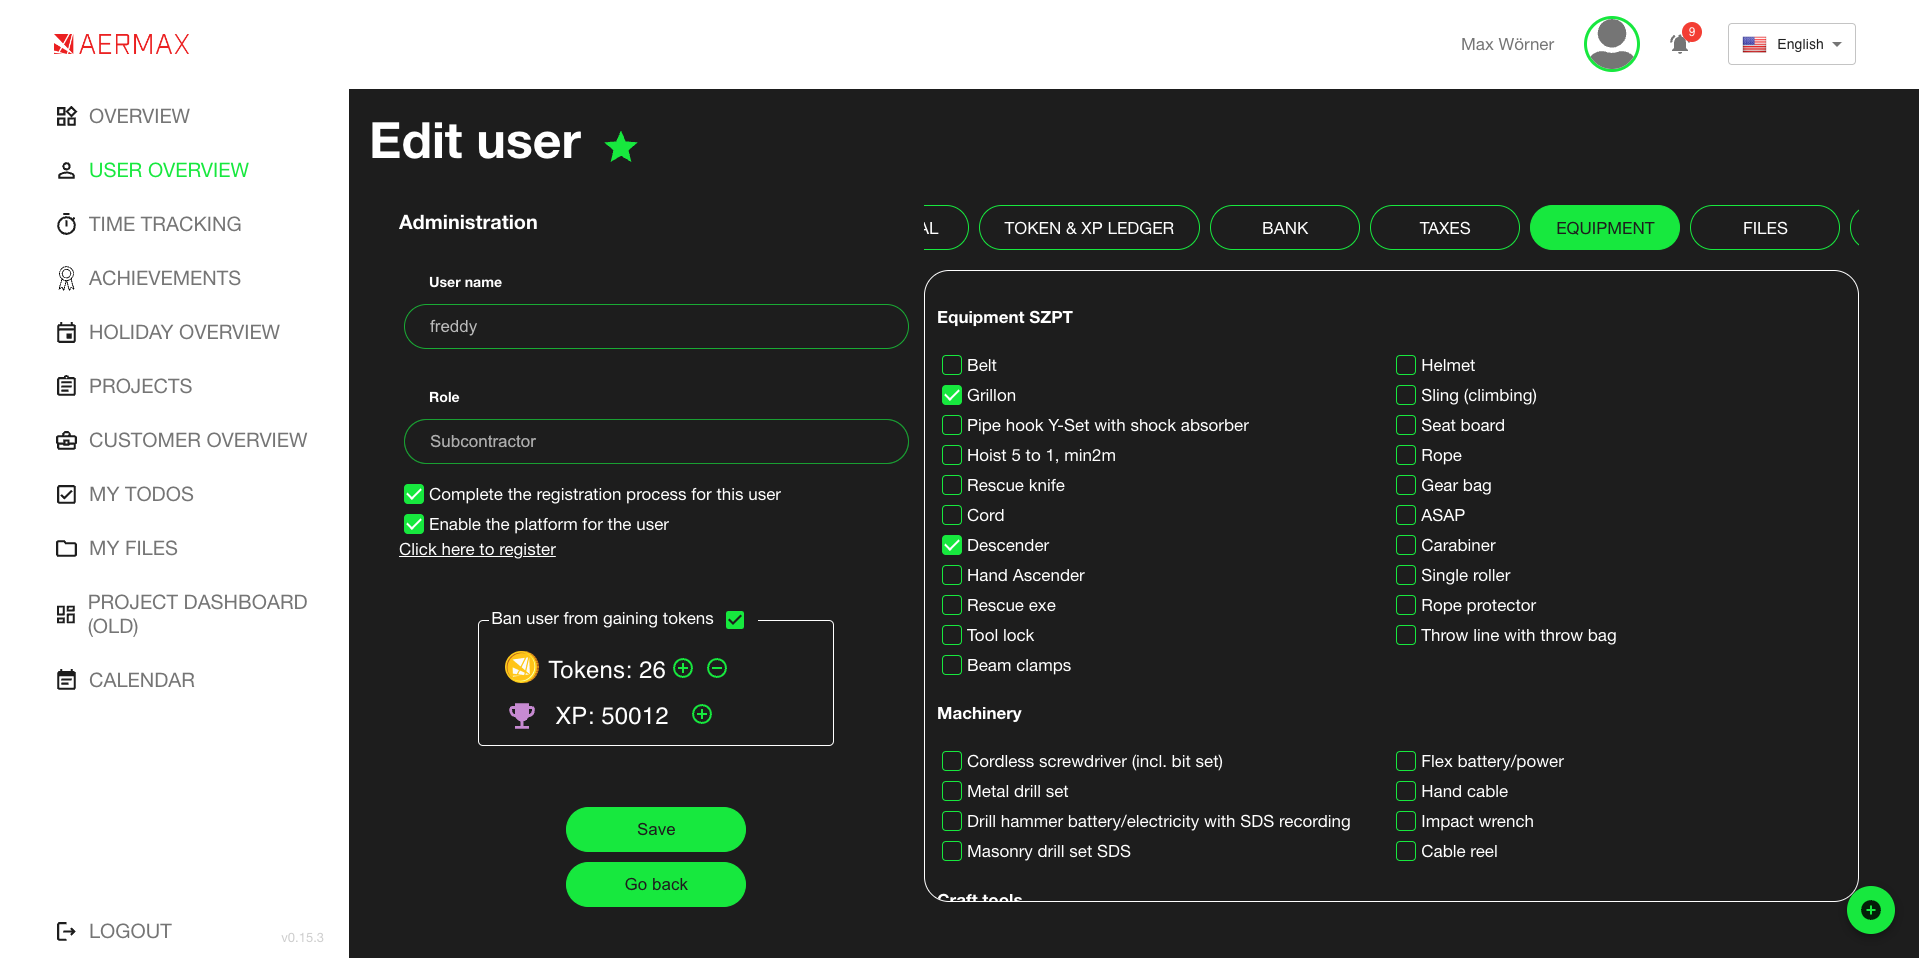
\includegraphics[width=0.9\textwidth]{src/assets/chapters/StaticDynamicEquipementList.png}
    \caption{Previous Static Equipment List}
    \label{fig:static_equipment_list}
\end{figure}

\subsubsection{Dynamic Equipment List}
To address these issues, we are transitioning to a dynamic equipment list. The dynamic implementation will automatically update the list based on changes in the equipment database, ensuring real-time accuracy and reducing maintenance overhead. Key features of the dynamic implementation include:
\begin{itemize}
    \item \textbf{Real-time Updates:} The list will automatically reflect changes made to the equipment database.
    \item \textbf{Improved Scalability:} The system can handle an increased number of equipment items without additional maintenance.
    \item \textbf{Enhanced User Experience:} Users will have access to up-to-date information, improving their ability to make decisions.
    \item \textbf{Reduced Maintenance:} Eliminates the need for manual updates, reducing the time and effort required to maintain the list.
    \item \textbf{Request System:} Subcontractors can request new equipment items directly through the system, allowing admins to approve, reject, and assign these items to appropriate groups.
\end{itemize}

The planned dynamic equipment list will also include comprehensive admin and subcompany views. As shown in Figure \ref{fig:dynamic_equipment_list_admin}, admins will have the capability to create groups, assign equipment, move equipment, and approve or reject equipment requests. Subcontractors, as illustrated in Figure \ref{fig:dynamic_equipment_list_subcompany}, will be able to write and request new equipment items, ensuring they have the necessary tools for their projects.

\begin{figure}[H]
    \centering
    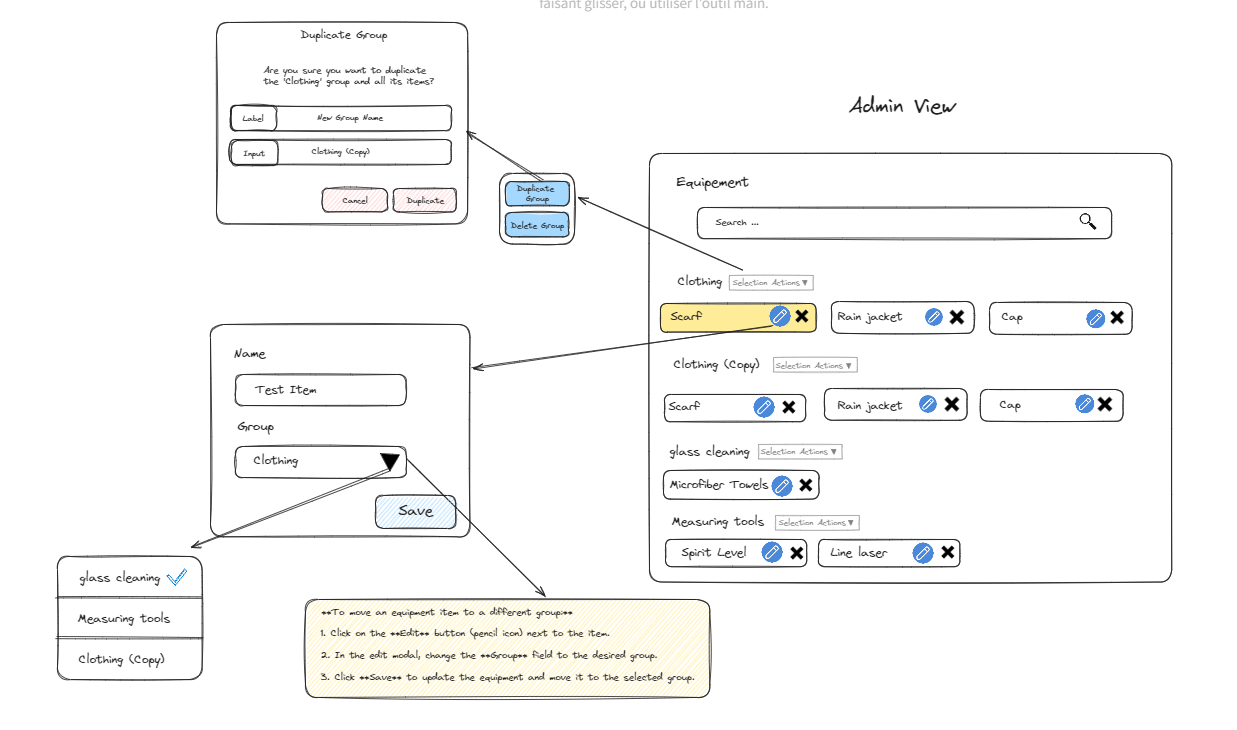
\includegraphics[width=1\textwidth]{src/assets/chapters/DynamicEquipementAdmin.PNG}
    \caption{Planned Dynamic Equipment List - Admin View}
    \label{fig:dynamic_equipment_list_admin}
\end{figure}

\begin{figure}[H]
    \centering
    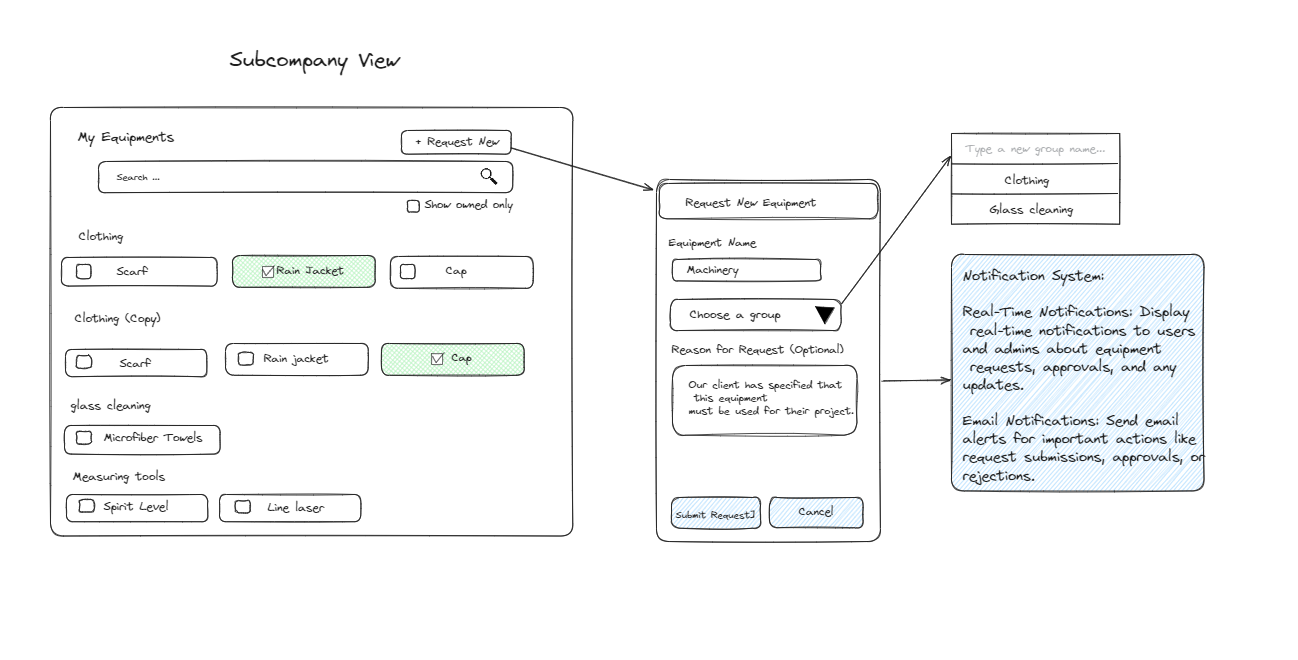
\includegraphics[width=1\textwidth]{src/assets/chapters/DynamicEquipementSubcompany.PNG}
    \caption{Planned Dynamic Equipment List - Subcompany View}
    \label{fig:dynamic_equipment_list_subcompany}
\end{figure}
\subsubsection{Dynamic Equipment Design}
To effectively transition from a static to a dynamic equipment list, we need to carefully design the system architecture. The dynamic system will facilitate real-time updates, scalability, and a user-friendly experience. The following sections provide a detailed overview of the class structure and interactions essential for implementing this dynamic equipment list.

The dynamic equipment list system will consist of several key components:

\begin{itemize}
    \item \textbf{Equipment Class:} This class will represent individual equipment items, including attributes such as name, group, status (requested, approved, rejected), and other relevant details.
    \item \textbf{Group Class:} This class will manage groups of equipment, allowing the creation, duplication, and deletion of groups. It will also handle the assignment and movement of equipment items between groups.
    \item \textbf{Request Class:} This class will handle equipment requests submitted by subcontractors. It will track the status of requests (pending, approved, rejected) and include details such as the equipment name and requested group.
    \item \textbf{User Class:} This class will manage user information, differentiating between admin and subcontractor roles, and providing appropriate permissions and functionalities for each role.
    \item \textbf{Notification System:} This component will handle real-time and email notifications to keep users informed about important actions like equipment requests, approvals, and rejections.
\end{itemize}
\paragraph{Class Diagram}
The class diagram below illustrates the key components and relationships involved in the dynamic equipment list feature.

\begin{figure}[H]
\centering
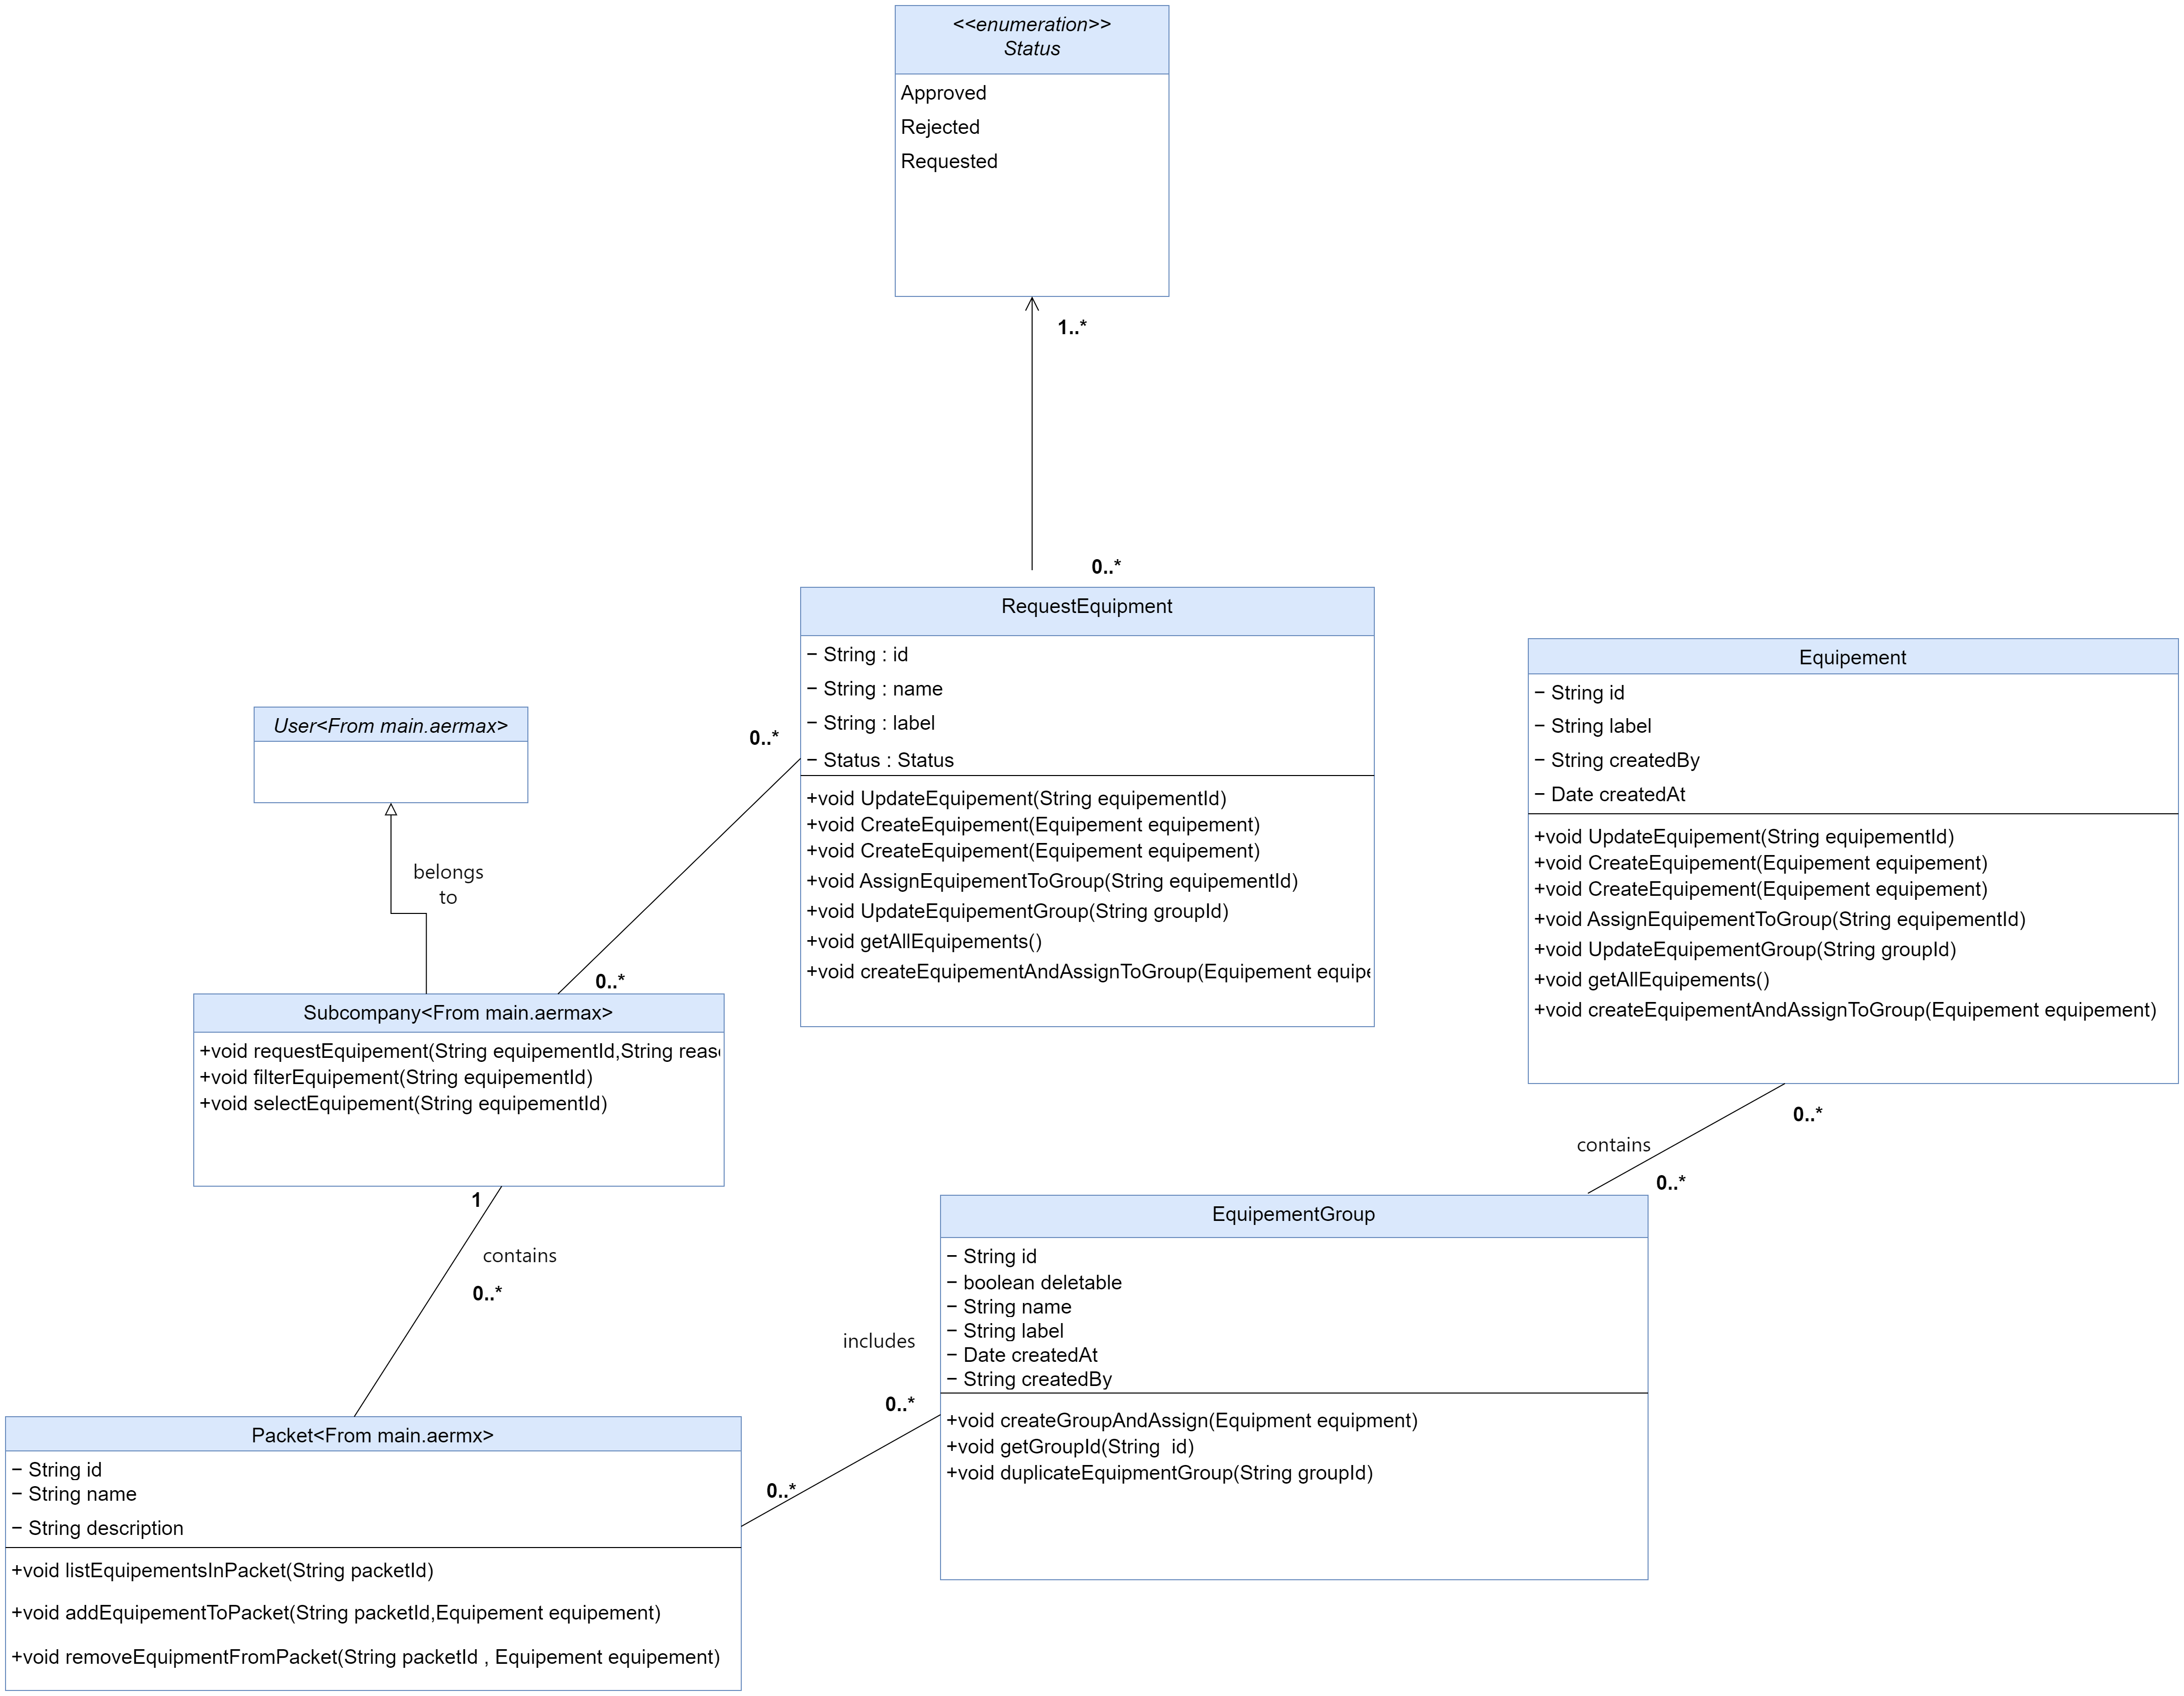
\includegraphics[width=1\textwidth]{src/assets/diagrams/DynamiEquipementListPng.png}
\caption{Class Diagram for Dynamic Equipment List}
\label{fig:class_diagram}
\end{figure}

\paragraph{Subcompany Interface}
The images below show the subcompany interface after the implementation of the dynamic equipment list, illustrating the improved user experience for subcompany users.

\begin{figure}[H]
\centering
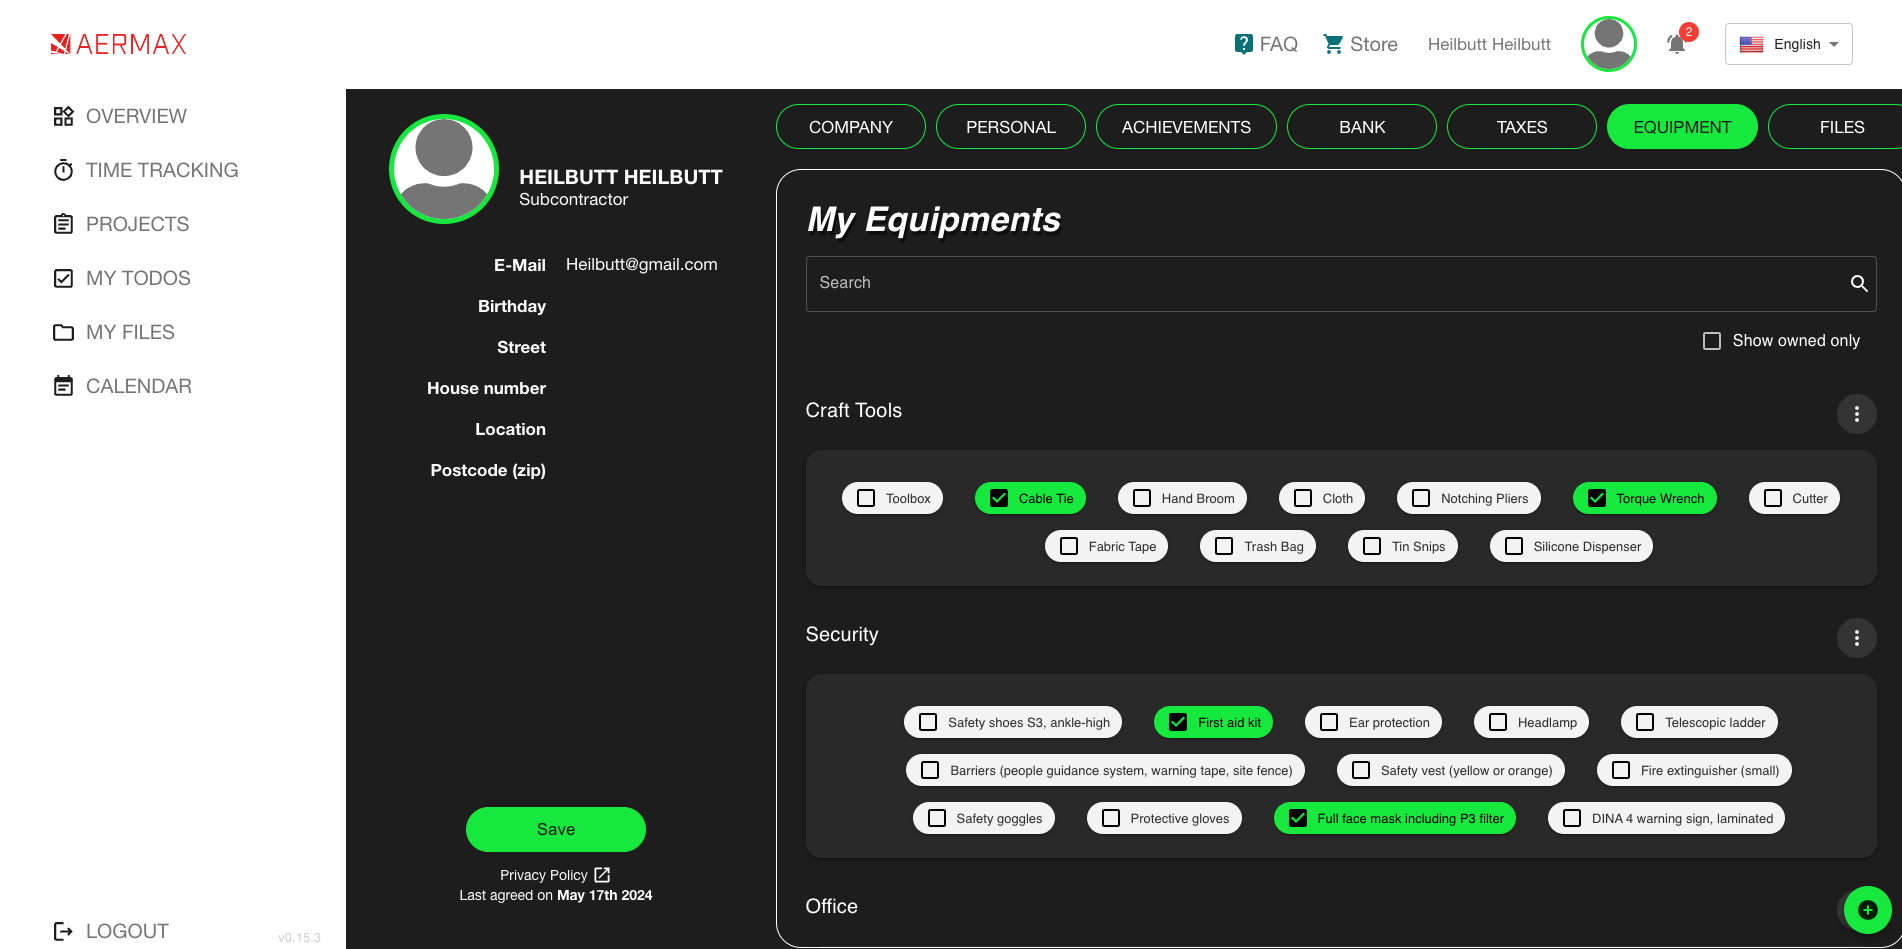
\includegraphics[width=0.9\textwidth]{src/assets/images/Interface1.png}
\caption{Subcompany Interface - Viewing Assigned Equipment}
\label{fig:subcompany_interface_1}
\end{figure}

\subsection{Adjust Feedback Notification}



\subsection{Overhaul of the Role System}
Before the Sprint 1 overhaul, the Aermax platform's role system was less delineated, with certain roles having either too broad or too narrow a range of permissions. This occasionally led to confusion, inefficiencies, and security concerns. For instance, Team Leaders had the same project creation rights as Administrators, and Workers had visibility into project overviews that were not relevant to their tasks.

After the Sprint 1 overhaul, we introduced a more refined role system, ensuring that permissions are tightly aligned with the responsibilities intrinsic to each role. The system was restructured to provide a balance between usability and security, reducing the cognitive load on users by limiting their interfaces to the features and information they need for their specific roles.

\subsubsection{Detailed Role Permissions Before \& After}
\begin{longtable}{|p{2.5cm}|p{2cm}|p{2cm}|p{2cm}|p{2cm}|p{2cm}|p{2cm}|p{3cm}|}
\caption{A before-and-after comparison of the detailed role permissions on the Aermax platform.} \label{tab:role_permissions_comparison} \\
\hline
\textbf{Role} & \textbf{View Packets Before} & \textbf{View Packets After} & \textbf{Create Projects Before} & \textbf{Create Projects After} & \textbf{Overview Feature Before} & \textbf{Overview Feature After} & \textbf{Additional Notes (After)} \\ \hline
\endfirsthead

\multicolumn{8}{c}%
{{\bfseries Table \thetable\ Continued from previous page}} \\
\hline
\textbf{Role} & \textbf{View Packets Before} & \textbf{View Packets After} & \textbf{Create Projects Before} & \textbf{Create Projects After} & \textbf{Overview Feature Before} & \textbf{Overview Feature After} & \textbf{Additional Notes (After)} \\ \hline
\endhead

\hline
\multicolumn{8}{|r|}{{Continued on next page}} \\ \hline
\endfoot

\hline
\endlastfoot

Administrator & All & All & Yes & Yes & Yes & Yes & Full system access \\ \hline
Employee & All & All & Yes & Yes & Yes & Yes & Administrative access \\ \hline
Project Manager & All & Specific & Yes & Yes (Start/Stop) & Yes & Yes & Administrative access; manage tasks, discussions, files \\ \hline
Worker & All & Own Only & Yes & No & Yes & No & Confined to personal scope of work \\ \hline
Team Leader & All & Phase Specific & Yes & No & Yes & No & Can view own packets and others within their phase; no project creation \\ \hline

\end{longtable}


% The following text can continue after the table in your LaTeX document.
\textbf{Scenario Demonstrations After Overhaul:}
\begin{itemize}
    \item \textbf{Administrator Scenario:} An Administrator maintains complete control, capable of managing all aspects of the project lifecycle.
    \item \textbf{Employee Scenario:} Employees continue to have similar administrative rights, including full packet visibility and project management capabilities.
    \item \textbf{Project Manager Scenario:} Project Managers are now provided with tailored access, capable of managing specific project packets and workflows.
    \item \textbf{Worker Scenario:} Workers are limited to their own packets, focusing their dashboard on personal tasks without additional project creation or overview privileges.
    \item \textbf{Team Leader Scenario:} Team Leaders have targeted oversight, managing only the packets within their project phase, without the distraction of other project overviews or creation capabilities.
\end{itemize}

This targeted approach in the role system refines the user experience on the Aermax platform, ensuring each role has the access needed to perform effectively, securely, and efficiently.

\subsection{Enhance Working Packets UI \& UX}
In our continuous efforts to elevate the user experience on the Aermax platform, a significant upgrade was made to the Working Packets UI \& UX, particularly focusing on the administrative interface. 

\begin{figure}[H]
    \centering
    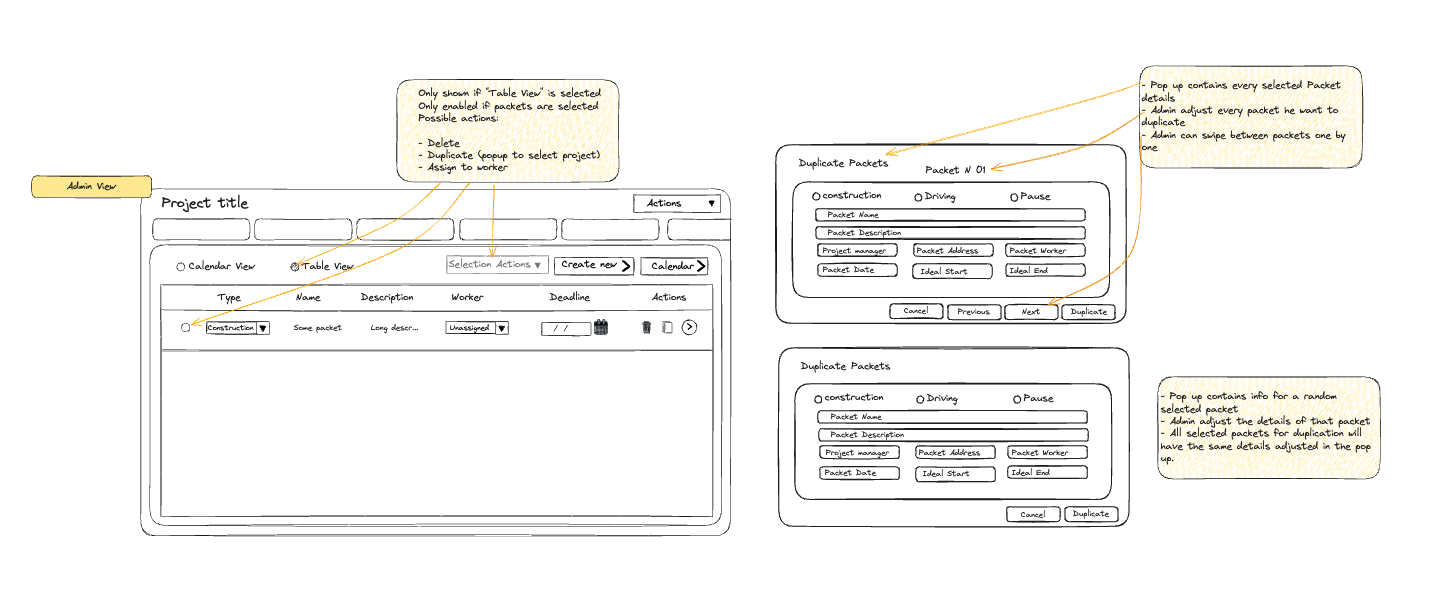
\includegraphics[width=1.1\textwidth]{src/assets/chapters/ui_ux-enhancement.png}
    \caption{Sketch of Planned UI/UX Enhancements for Working Packets }
    \label{fig:ui_ux_enhancements}
\end{figure}


\begin{figure}[H]
    \centering
    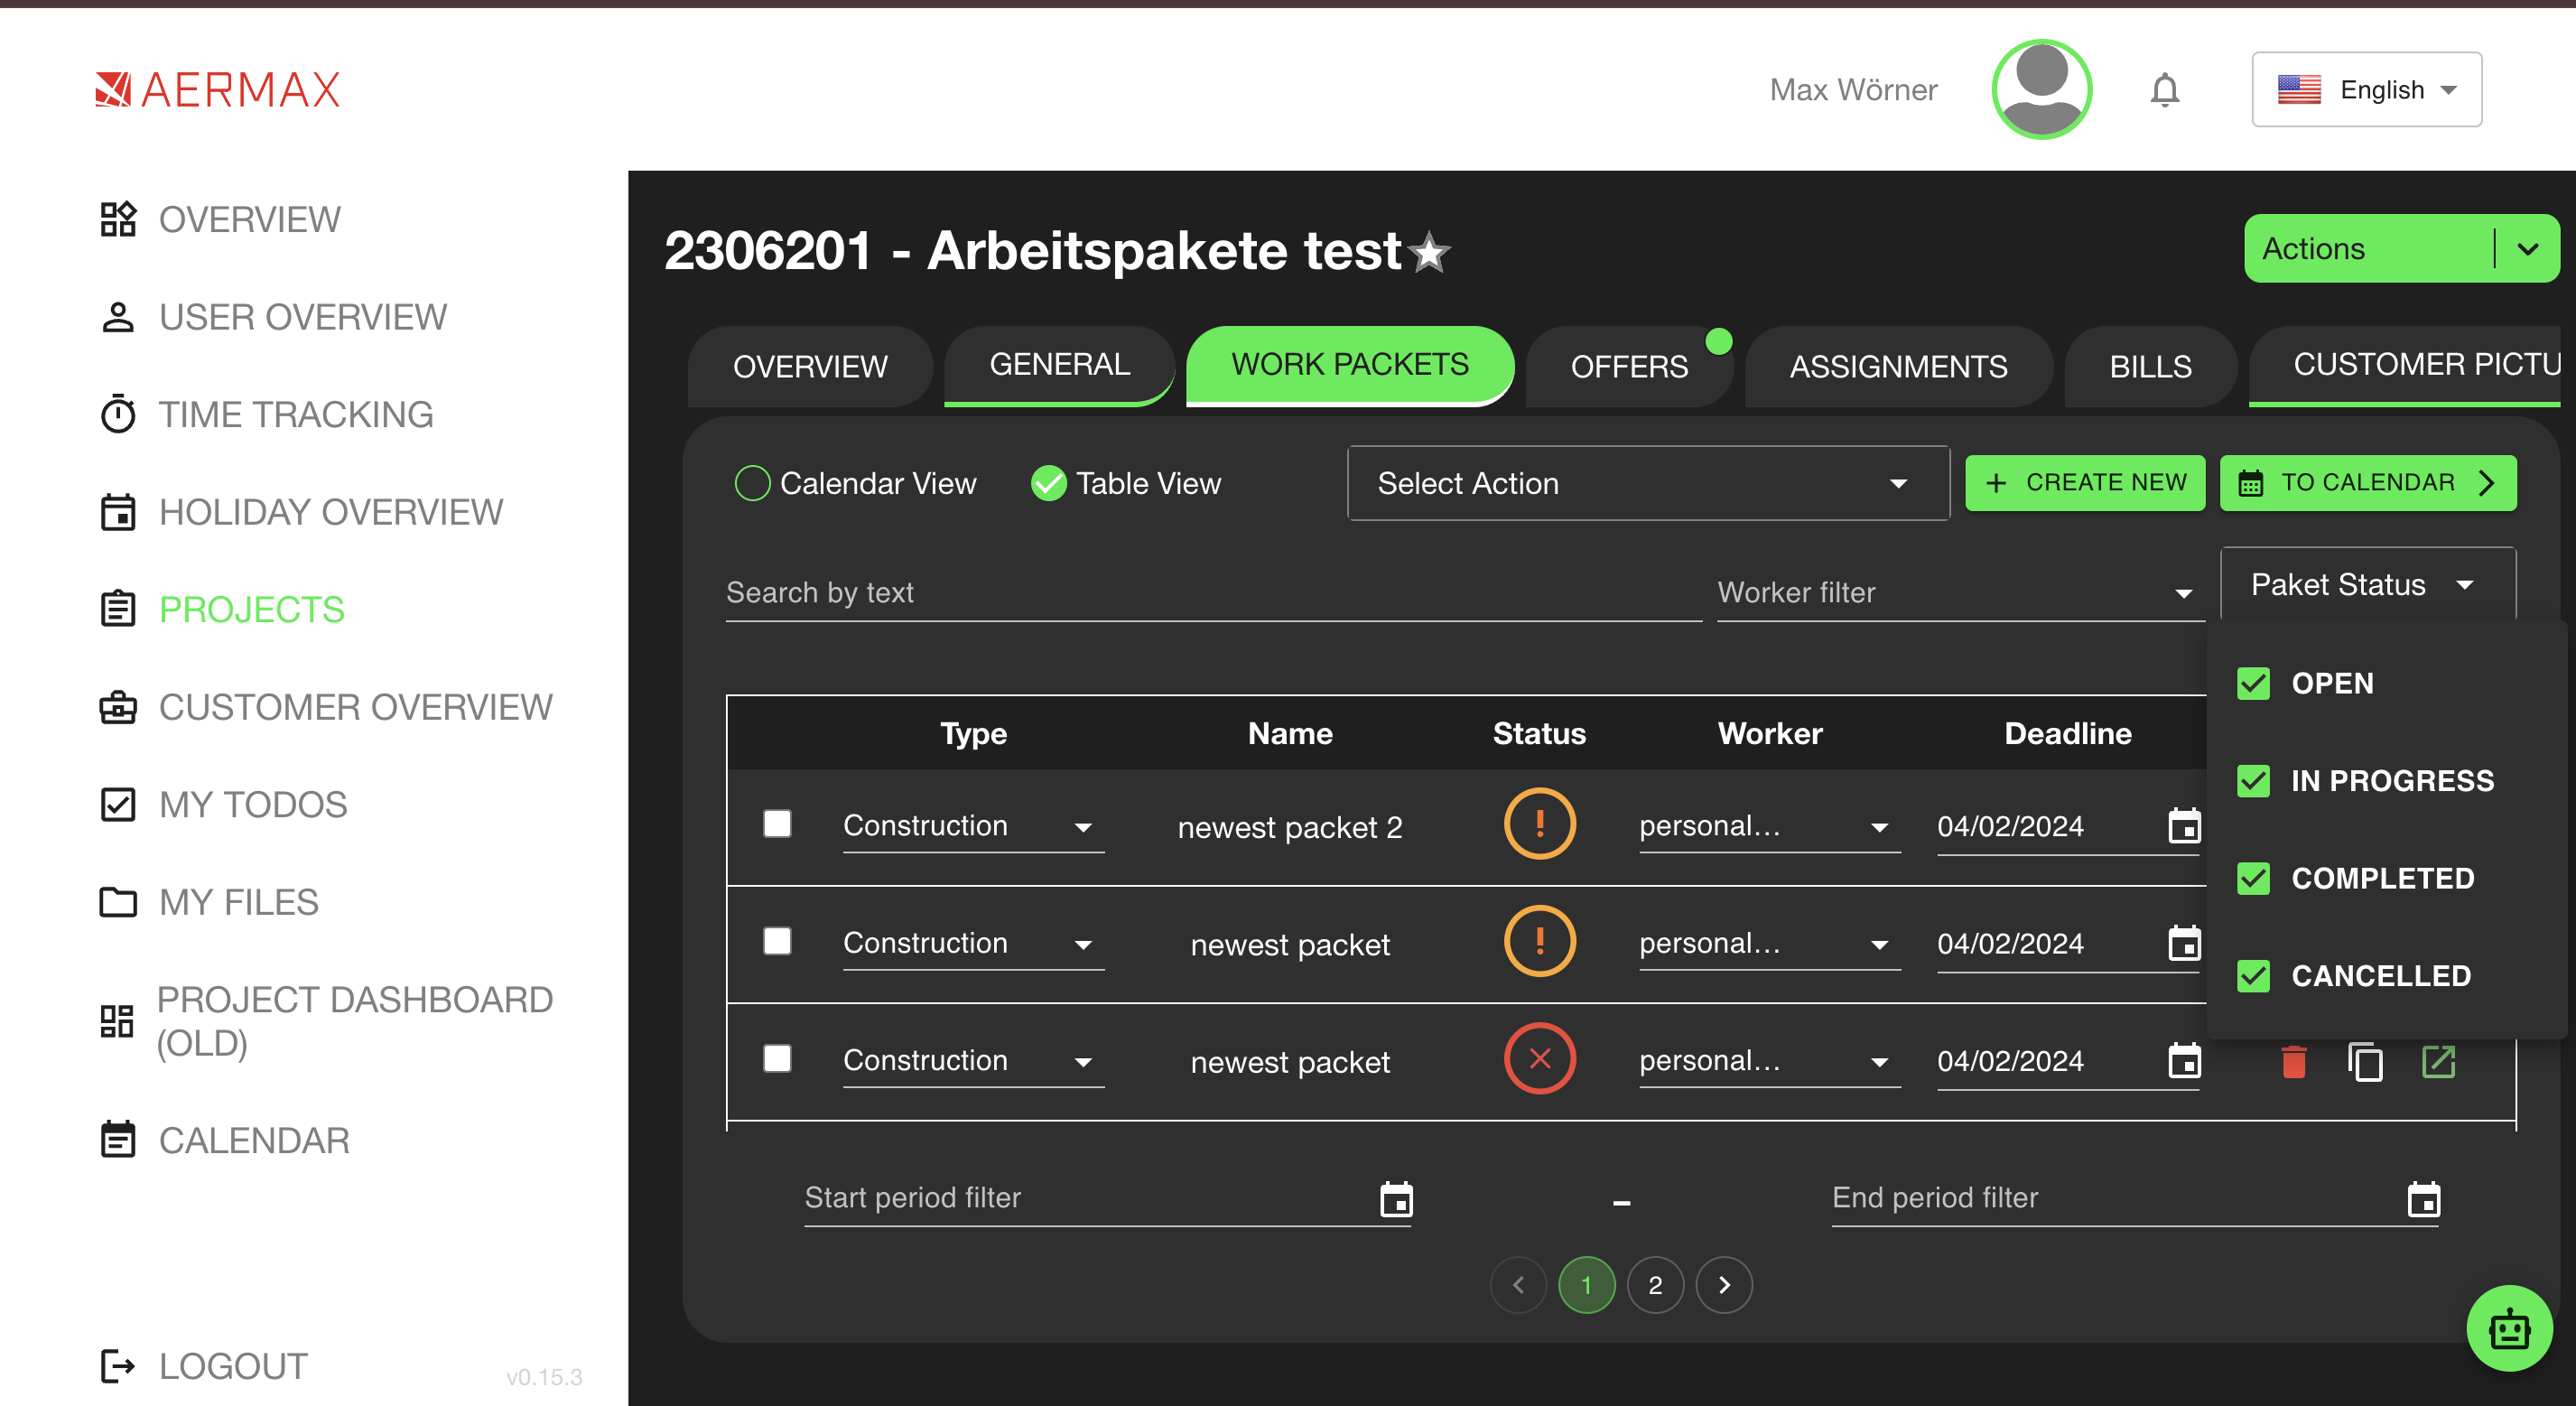
\includegraphics[width=0.9\textwidth]{src/assets/chapters/newTable1.png}
    \caption{Sketch of Planned UI/UX Enhancements for Working Packets }
    \label{fig:ui_ux_enhancements}
\end{figure}


\begin{figure}[H]
    \centering
    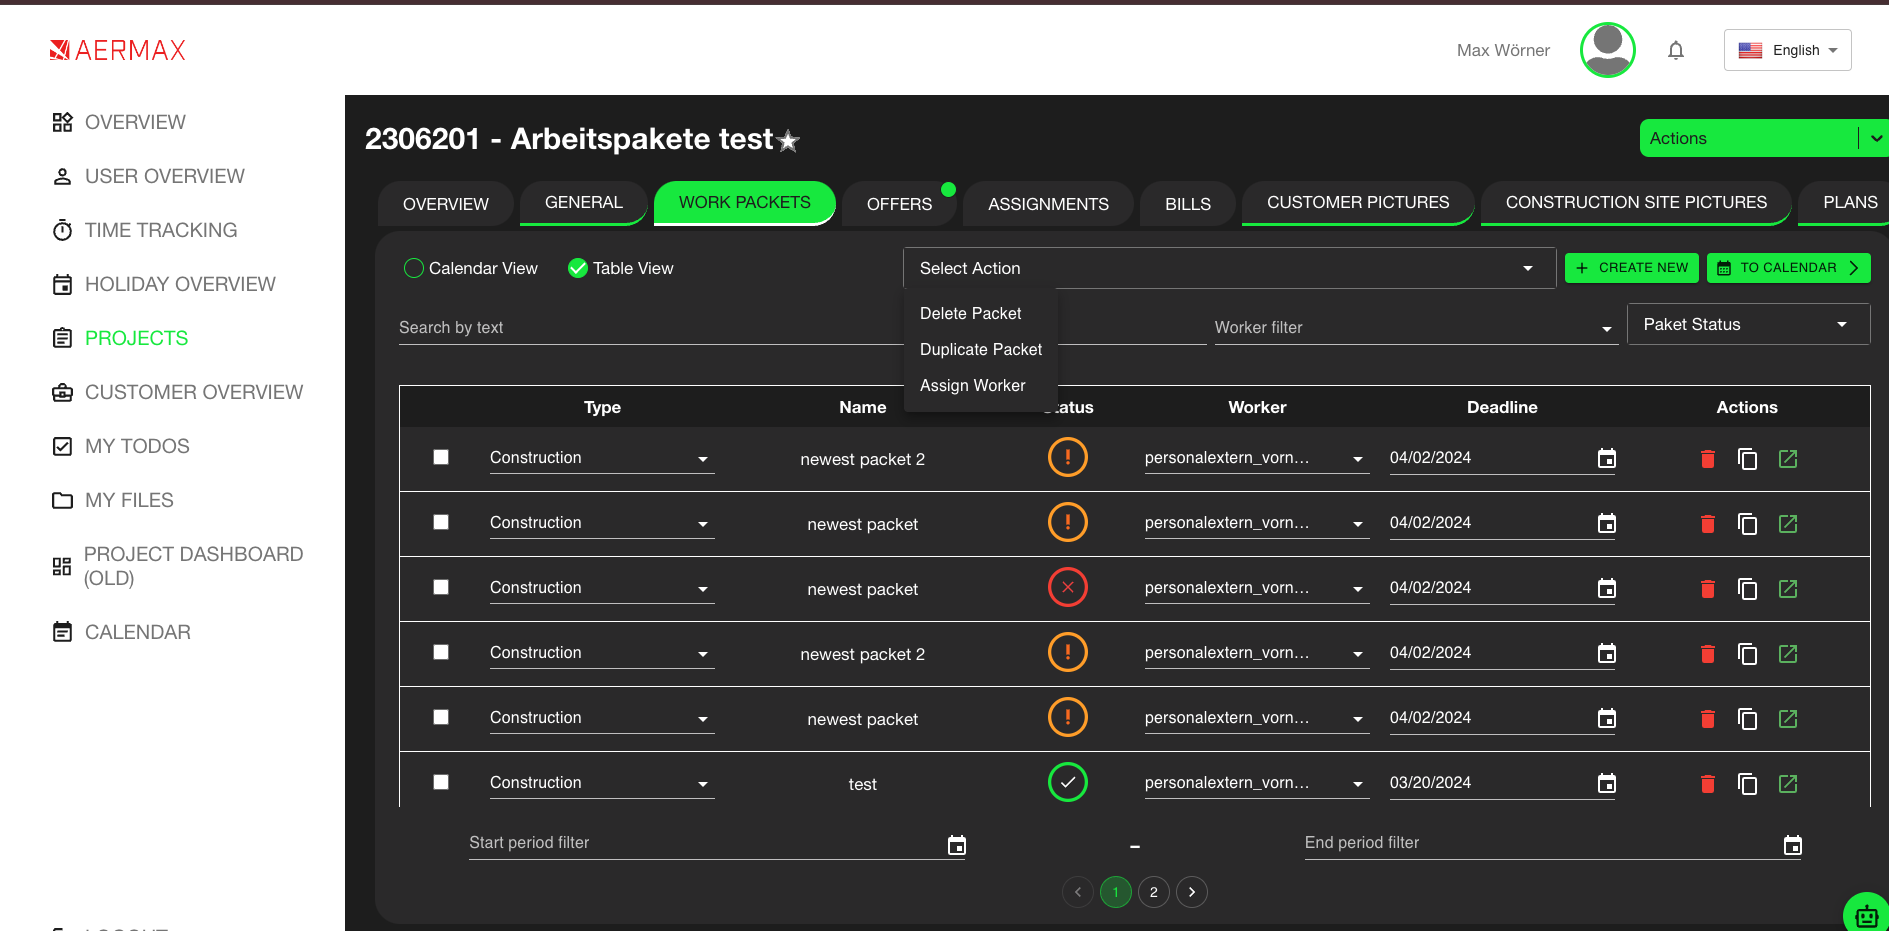
\includegraphics[width=0.9\textwidth]{src/assets/chapters/newTable2.png}
    \caption{Sketch of Planned UI/UX Enhancements for Working Packets }
    \label{fig:ui_ux_enhancements}
\end{figure}

\subsection{Self Registration}

We have implemented a self-registration feature that streamlines the process of user registration, allowing new users to create accounts autonomously.

\begin{figure}[H]
    \centering
    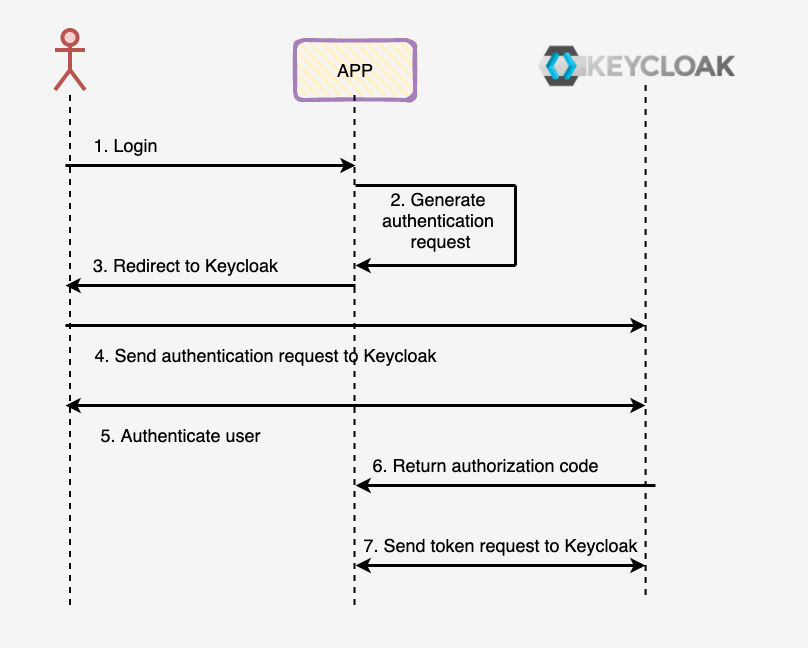
\includegraphics[width=0.9\textwidth]{src/assets/chapters/keycloak-diagram.png}
    \caption{Authentication Flow Using Keycloak: A visual guide to the user authentication process with Keycloak.}
    \label{fig:authentication_flow_keycloak}
\end{figure}

Figure \ref{fig:authentication_flow_keycloak} illustrates the authentication flow using Keycloak. The figure will show the step-by-step authentication flow, demonstrating how users interact with Keycloak during the login process. It provides a visual explanation of the authentication steps from the user initiating a login request to receiving a token from Keycloak.

As part of this overhaul, we encountered the challenge of duplicate user entries due to previous system design limitations. By leveraging Keycloak’s versatile user federation and identity provider features, we were able to consolidate user accounts and eliminate redundancies, thereby solving the issue of duplicate entries. 

Keycloakify complemented this integration by allowing us to customize the authentication pages to align with our platform's aesthetics and usability standards.

\subsubsection{Feature Implementation Table:}
\begin{table}[H]
\centering
\begin{tabularx}{\textwidth}{|X|X|X|}
\hline
\textbf{Feature} & \textbf{Technology Implemented} & \textbf{Description} \\
\hline
Login/Signup & Keycloak, Keycloakify & Integrated with Keycloak to secure and streamline user access, enhanced by Keycloakify for customized UI/UX. \\
\hline
Password Management & Keycloak & Developed a secure and user-friendly password management system, providing users with ease of control over their credentials. \\
\hline
\end{tabularx}
\caption{Summary of Keycloak feature implementations.}
\label{tab:keycloak_features}
\end{table}

\subsection{Backend Enhancements and Data Integrity}
\textbf{Eliminating Duplicate Users and Improving Data Handling}
Our backend team undertook the critical task of enhancing the database and data processing layers of our system. The focus was on refining our data model to eliminate the occurrence of duplicate user entries—a problem that stemmed from a legacy design.
 
\begin{figure}[H]
    \centering
    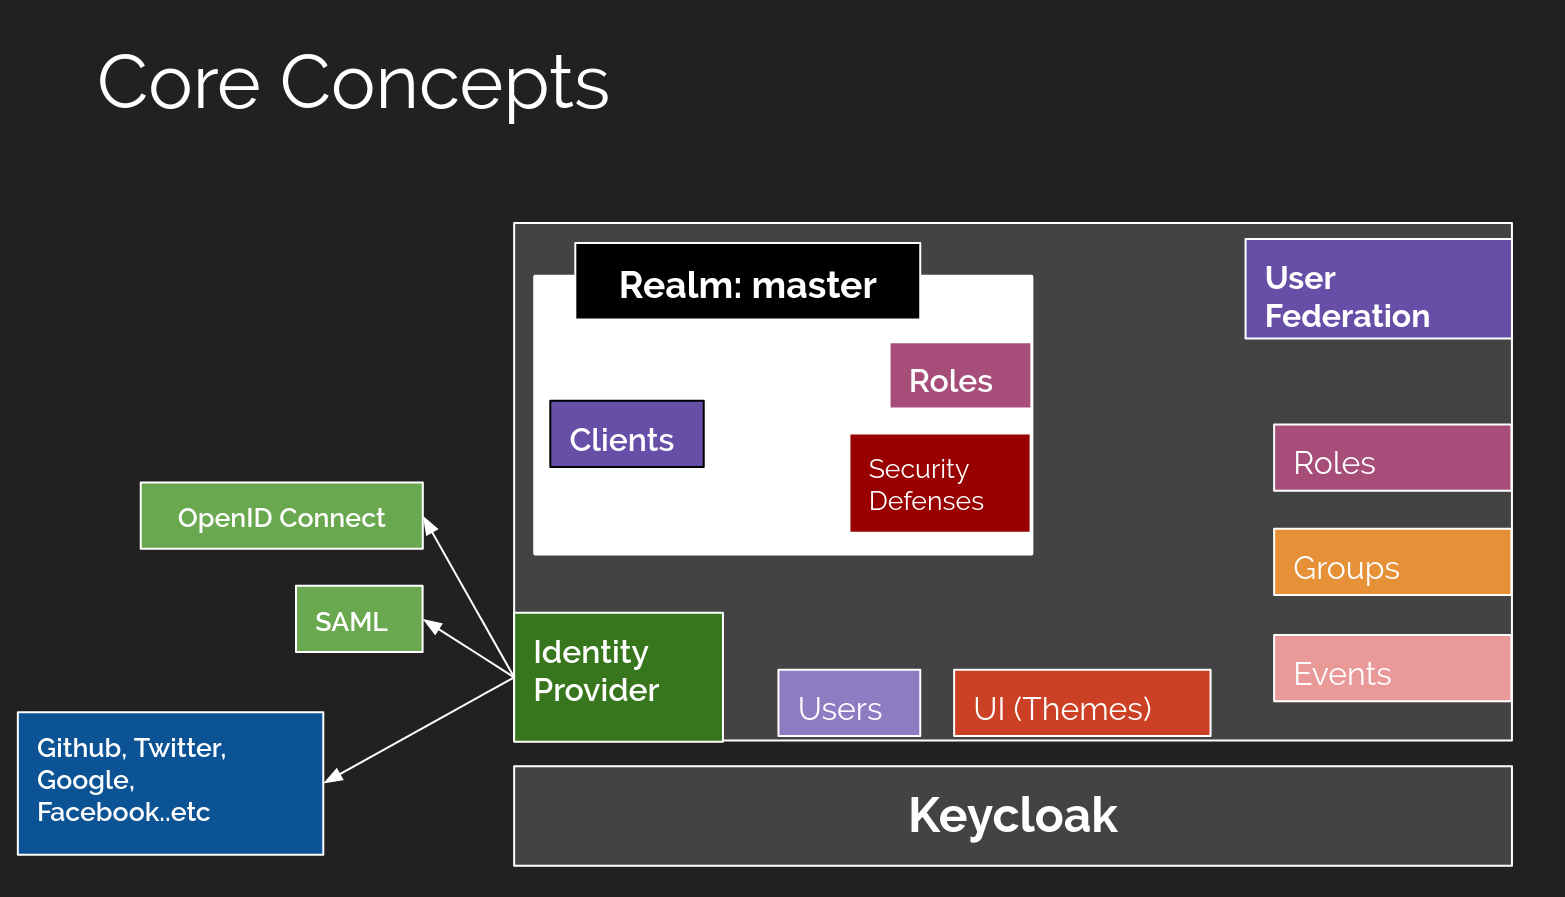
\includegraphics[width=0.9\textwidth]{src/assets/chapters/core-conccept.png}
    \caption{Core Concepts of Keycloak's Architecture}
    \label{fig:core_concepts_keycloak}
\end{figure}

This image will give an overview of Keycloak’s core concepts, such as realms, roles, and identity providers. It visually communicates the architecture that supports the functionality we harnessed to solve our data integrity challenges.


\subsection{UI/UX Design Improvements}
\addcontentsline{toc}{subsection}{UI/UX Design Improvements}
With user experience at the forefront of our digital solution, the Aermax platform underwent a significant UI/UX redesign to enhance cleanliness, intuitiveness, and functionality. Using Figma, our design team was able to collaborate on and iterate high-fidelity mockups and prototypes, which provided a visual roadmap for the platform's evolution.

\textbf{Objective:} To revamp the Aermax platform's design for a more streamlined, user-friendly interface that aligns with modern standards and enhances user engagement.

\textbf{Outcome:} The design overhaul has resulted in a cleaner and more intuitive interface that simplifies user interactions and reduces cognitive load. With a focus on ease of use, the new design has improved the overall user experience, leading to increased user satisfaction and platform adoption.

\textbf{Visual Demonstration:} The following images compare the original and the new Figma-enhanced UI/UX designs, showcasing the transformation and the design team's dedication to creating a user-centred interface.

 

\begin{figure}[H]
    \centering
    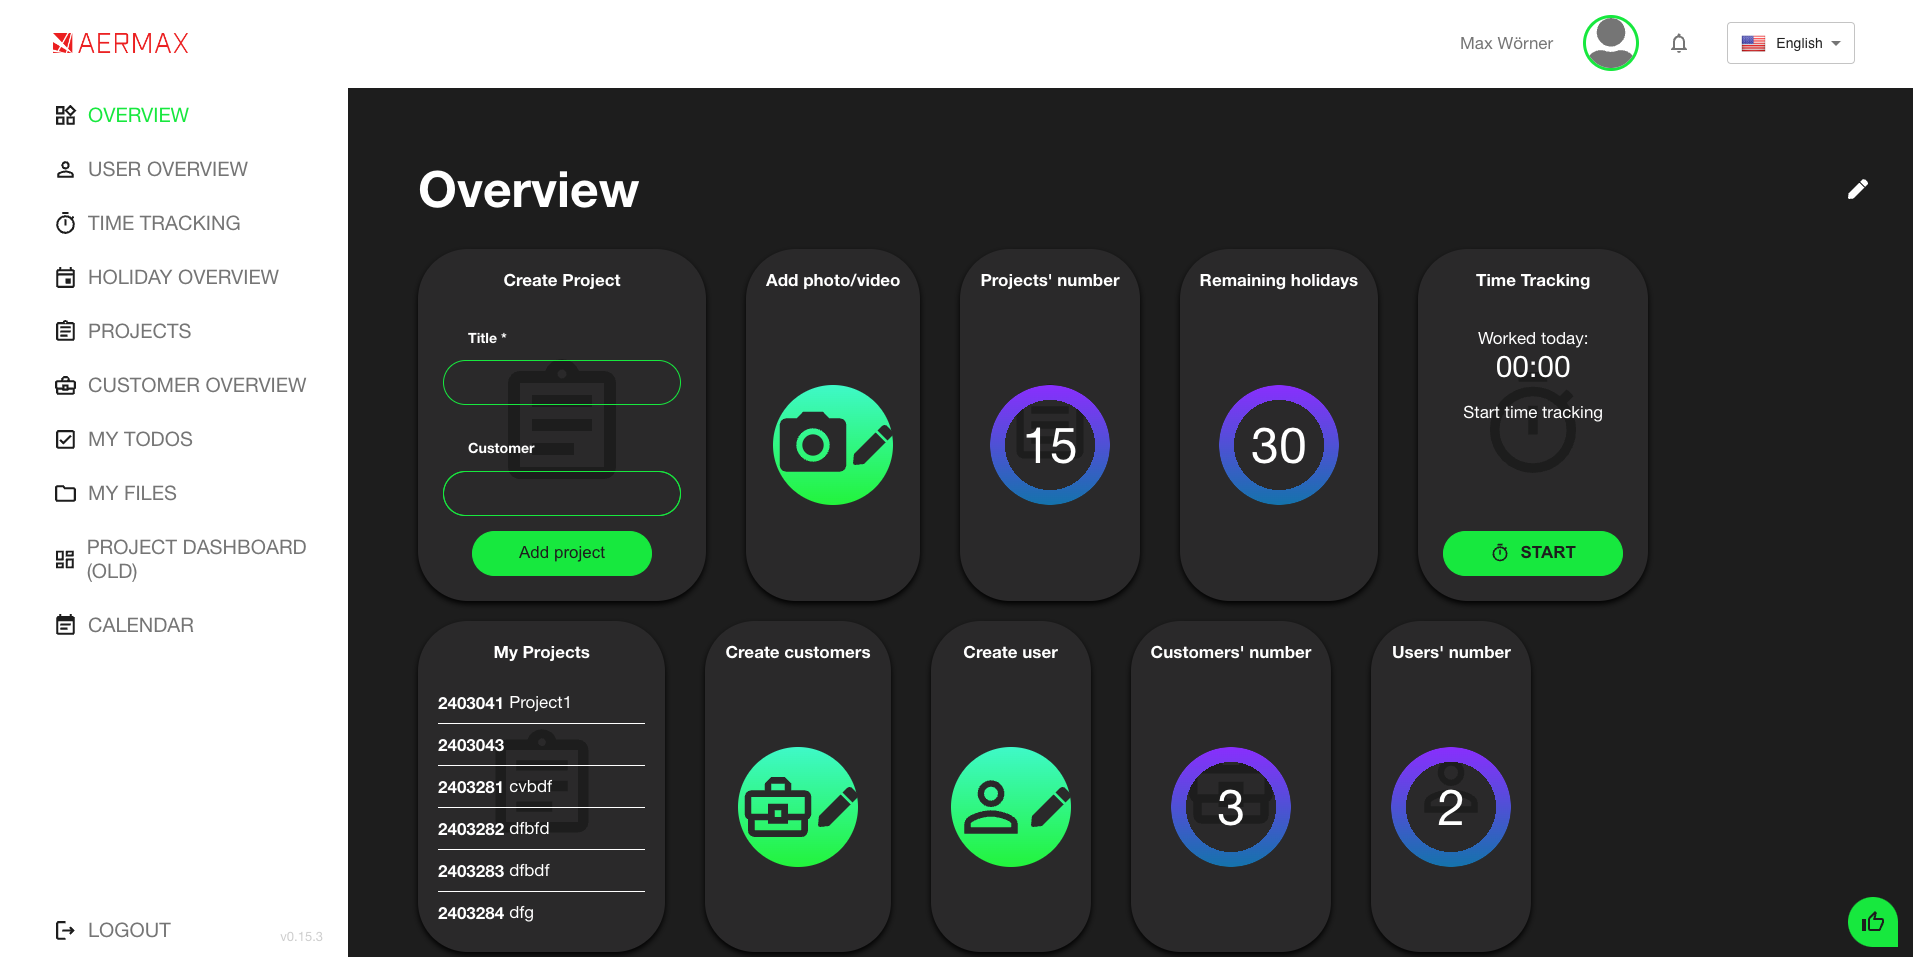
\includegraphics[width=0.9\textwidth]{src/assets/chapters/OverviewPage.png}
    \caption{Original Aermax platform Overview page UI design.}
    \label{fig:overview_page_design}
\end{figure}

\begin{figure}[H]
    \centering
    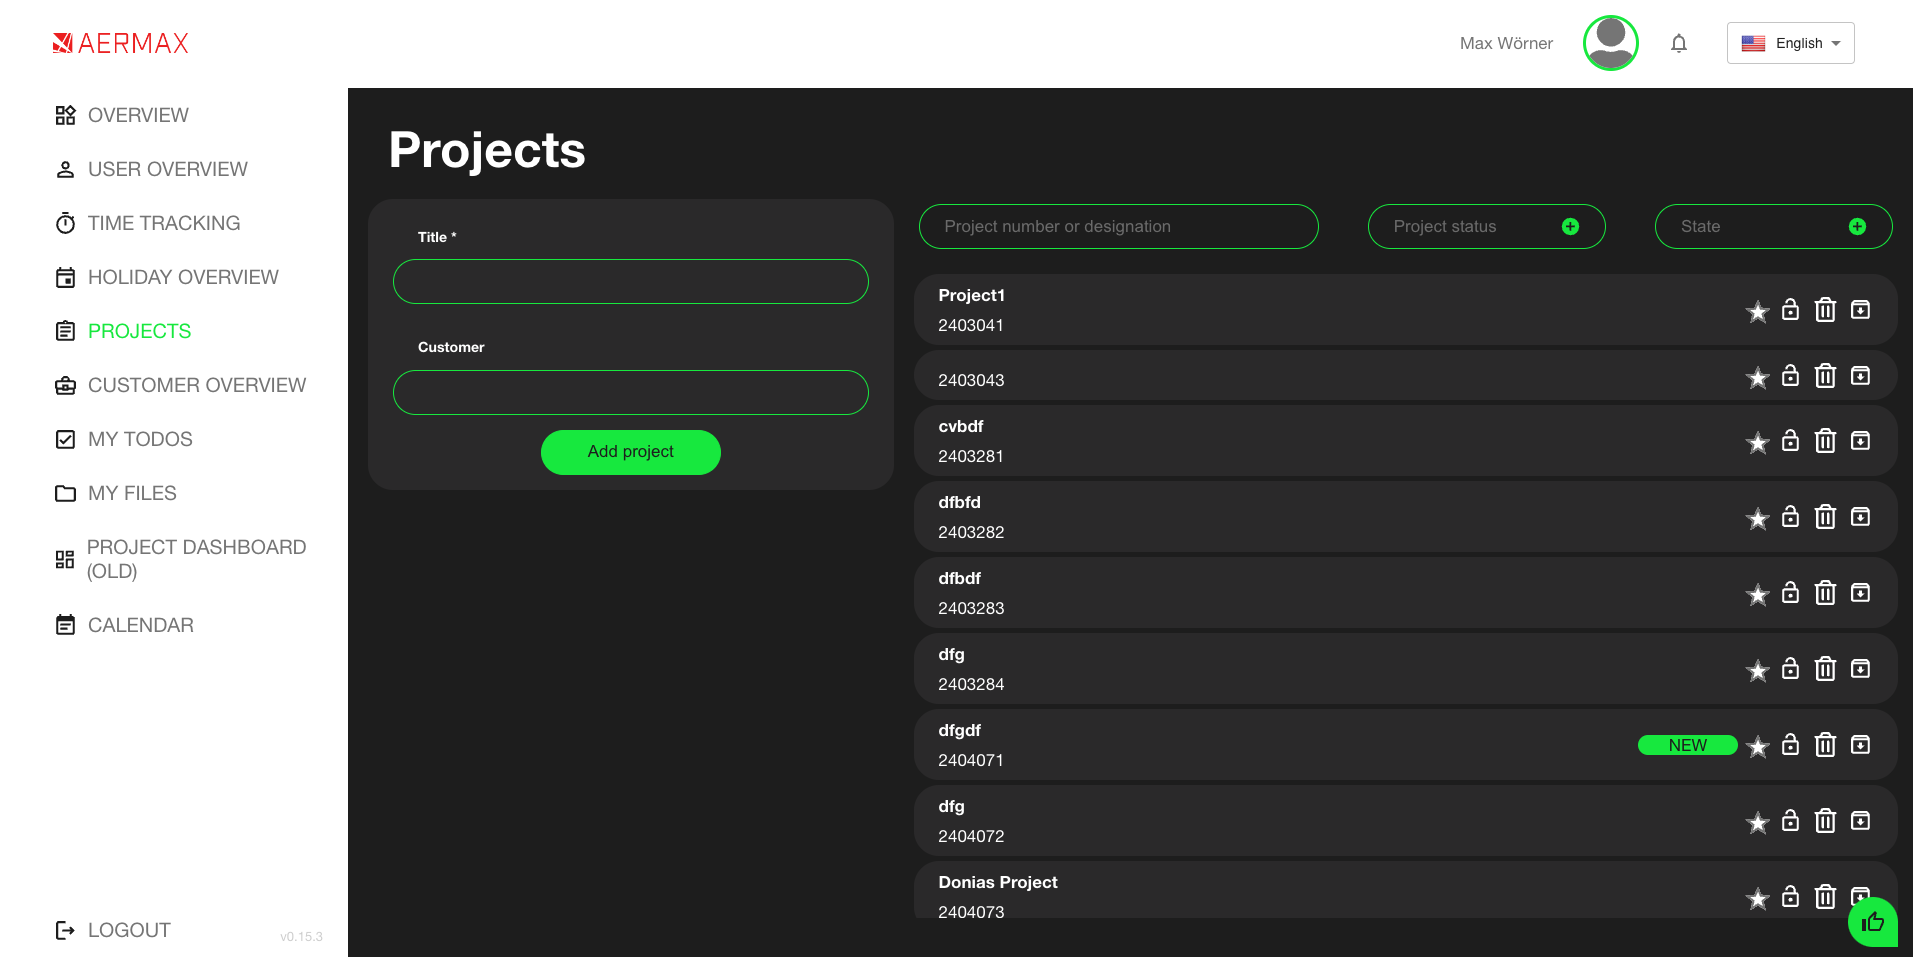
\includegraphics[width=0.9\textwidth]{src/assets/chapters/ProjectPage.png}
    \caption{Original Aermax platform Project page UI design.}
    \label{fig:project_page_design}
\end{figure}


\begin{figure}[H]
    \centering
    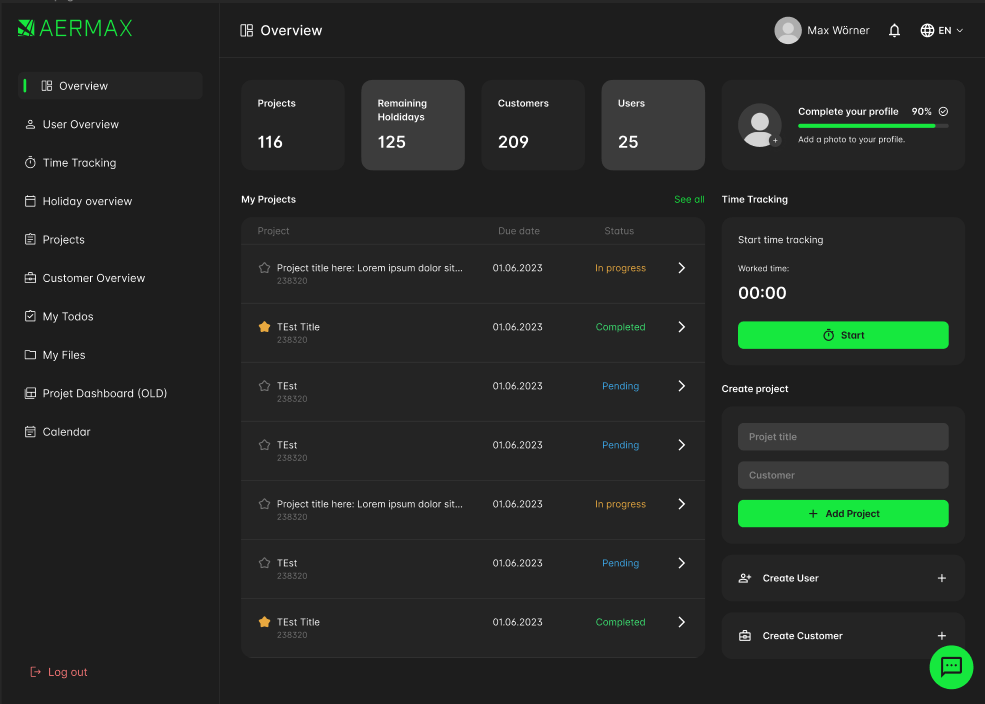
\includegraphics[width=0.9\textwidth]{src/assets/chapters/ui-ux-dashboard.png}
    \caption{Enhanced Aermax platform Overview page UI design in dark mode.}
    \label{fig:enhanced_overview_dark}
\end{figure}

\begin{figure}[H]
    \centering
    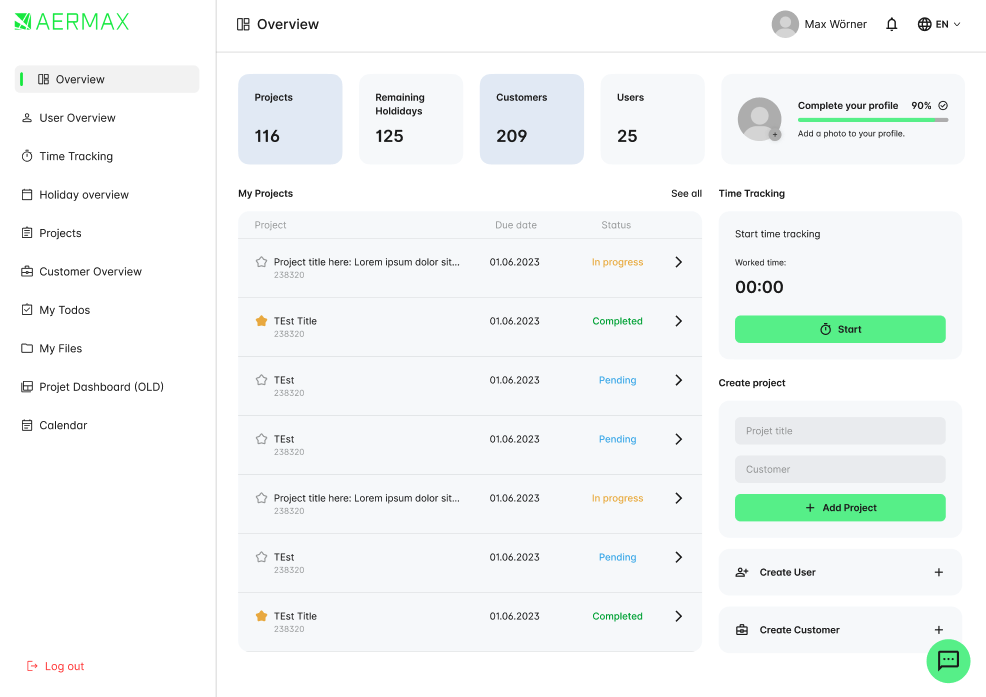
\includegraphics[width=0.9\textwidth]{src/assets/chapters/ui--ux-dashboard.png}
    \caption{Enhanced Aermax platform Overview page UI design in light mode.}
    \label{fig:enhanced_overview_light}
\end{figure}

\begin{figure}[H]
    \centering
    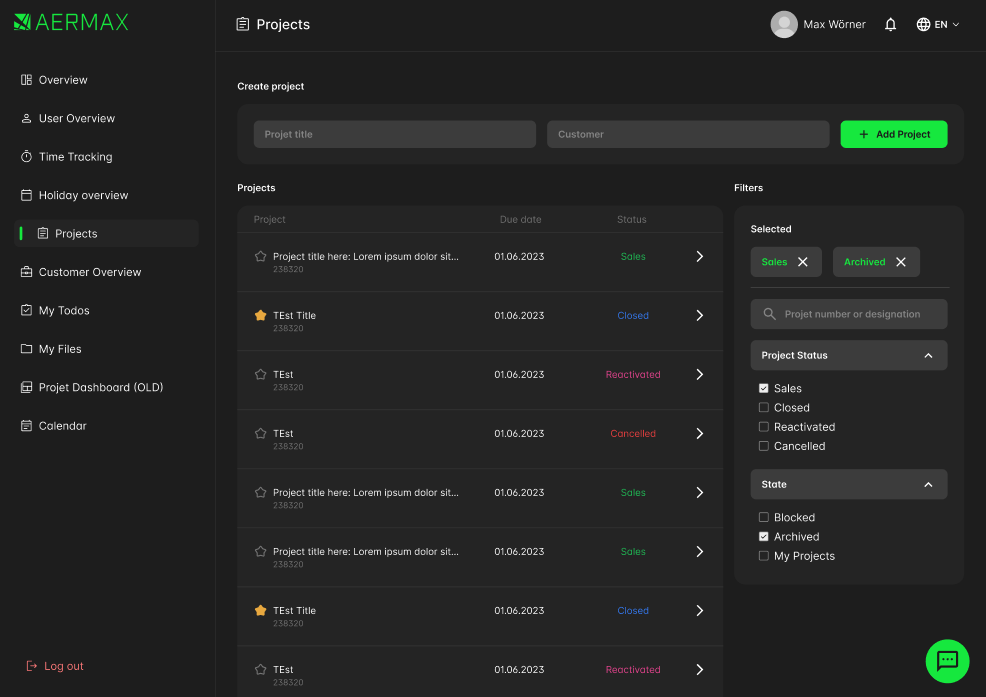
\includegraphics[width=0.9\textwidth]{src/assets/chapters/ui-ux--peoject.png}
    \caption{Enhanced Aermax platform Project page UI design.}
    \label{fig:enhanced_project_page}
\end{figure}

